
\include{Preamble}

\usepackage{circuitikz}
\usepackage{pdflscape}

%The title page
\title{EMB1 - Project 2\\ The Quadrocopter \rule{14cm}{0.5mm}}
\author{Rolf Green -- rogre11@student.sdu.dk\\ 
	Malthe Høj-Sunesen -- mhoej10@student.sdu.dk\\ 
	Krzysztof Smyl -- krsmy14@student.sdu.dk\\ 
        \rule{14cm}{0.5mm}}
\date{Submission date: 2014-12-19}


\begin{document}
%\setlength{\parindent}{0pt} %no indent
%
\pagenumbering{gobble}% removes page numbers
\maketitle %Makes the title
\begin{figure}[H]
\centering
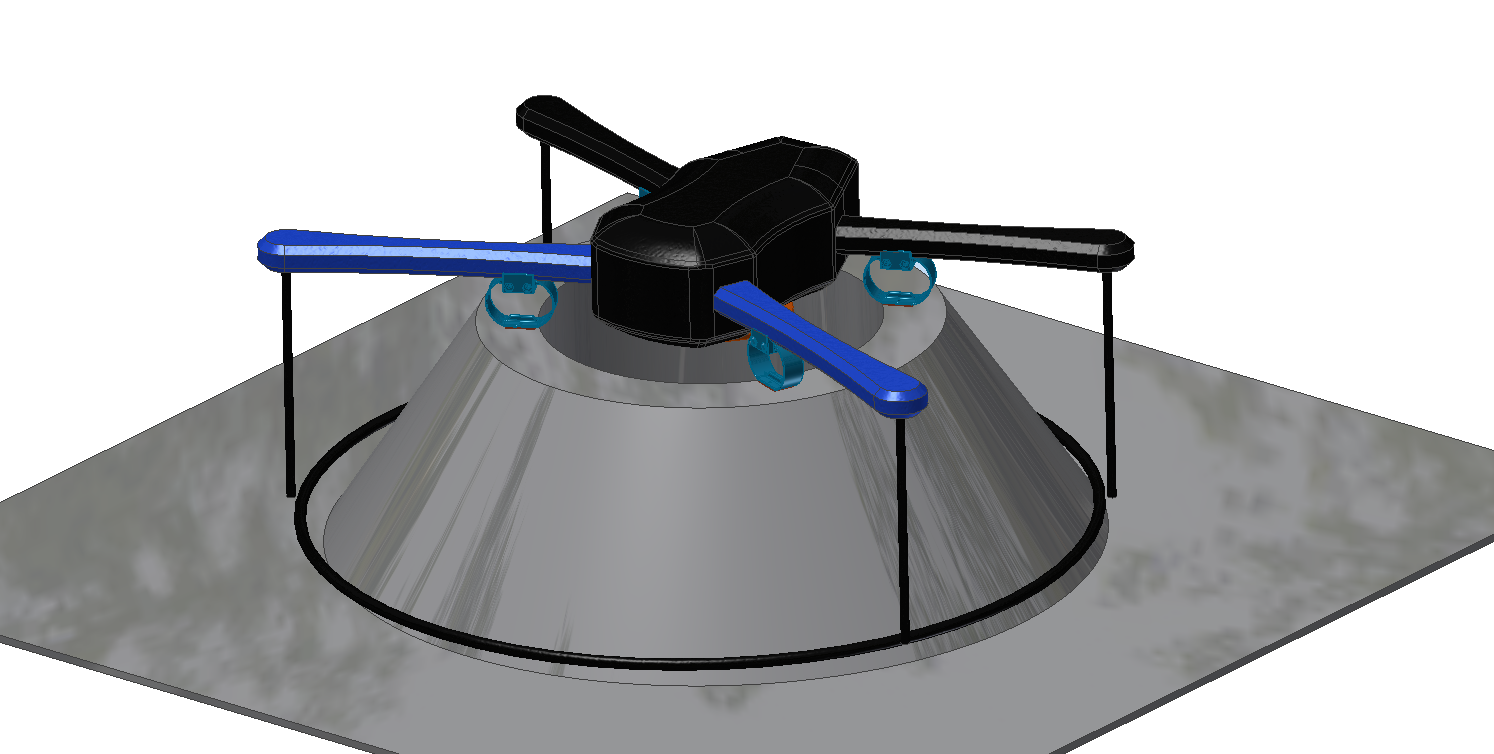
\includegraphics[width=0.9\textwidth]{introduction/frontpage}
\caption{The Quadrocopter}
\label{fig:frontpage}
\end{figure}
\begin{center}
Pages: \pageref{LastPage}
\end{center}
\newpage % Makes a new page
\newpage
\pagenumbering{arabic} % Makes pages numbers and resets them to 1
\pagestyle{fancyplain}
\fancyhf{}
%
\lhead{ \fancyplain{}{Syddansk Universitet - EMB1} } % left page header
%
%
\rfoot{ \fancyplain{}{Page \thepage\ of \pageref{LastPage}} }
\begin{abstract}
This report describes the development of a UAS that allows a UAV to take off, fly a preprogrammed route if conditions allow flying, return to the base by GPS and then be guided via computer vision to land and recharge on a ground base. This system is not fully developed but the steps towards is described in this report. 

A physical landing platform was developed. Two designs were in consideration and an analysis of the two is made. The landing platform shaped as a cone was chosen as the best solution. Test were made to ensure that the UAV would slide correctly into place. A real prototype of the platform were made. Connector pods were designed, tested and redesigned. The prototype was equipped with LEDs to show connections to the pods. The physical platforms works well, but is just a prototype and materials and design needs to be refined. 

The computer vision guiding was designed using the ROS framework. This was found to make testing of multiple tracking methods and testing with recorded video easier. Three different tracking methods for location the UAV in the image were tested.  Only one of these were performing useful in a outdoor environment, due to difficult light conditions. A method for calculating the position of the UAV 3D position relative to the camera, in SI units, was also developed. The 3D position made it possible to visualize the drone in the RobWorkStudio 3D simulator. The tracking is still just a prototype but ended up being a nice proof of concept. 

The firmware for a IRIS drone with Pixhawk was examined. Both APM and Pixhawk flight stack were used to do test flights. They were found equally good, when calibration was done correctly. Different flight modes for Pixhawk was examined and auto, AltHold and land was found best suited for making use in automatic landing. A script for using METAR and TAF messages for automatic weather forecasts was found. The use of MAVRos for controlling the UAV was examined and the RCOverride method was found useful. Pseudocode for an automatic landing system was shown.

The whole system was not tested together as the subtasks was not finished. Future work should is to finish the subtasks and build them together into one system. 
\end{abstract}
\newpage
\tableofcontents
\newpage
%
\section{Introduction} \label{chap:intro}
\section{Introduction}
\subsection{Project background and scope}
In many applications, primarily in agriculture, an autonomous UAV which can follow a pre programmed route and return to a base to recharge like an autonomous lawn mower, is sought after. One case could be a farmer. As the legislation is now the farmer must daily inspect his animals. This prevents the use of some remote areas which is otherwise perfect for the farmer’s use; as small islands or remote field with good grass. Areas that take time, money or effort to get to in order to inspect the animals.
Our vision is to develop a system which allows a UAV to take off, fly a pre programmed route if conditions allow flying, return to the base by GPS and the guided via GNSS/Computer Vision land to recharge on a ground base. Then the UAV will be ready for next flight the next day..
\subsection{Problem formulation}
The problems in this project will be to:

\begin{itemize}
	\item Modify Pixhawk firmware to be controlled automatically from an external computer;
	\item Build/design/construct a landing-platform with mechanical autofit;
	\item Design a tracking-system that outputs 3D-positions; and,
	\item Design a program that analyze 3D-positions and outputs control-signals.
\end{itemize}

\subsection{Related work}
XX DYLAN?
XX LASER GUIDED?

\subsection{Hypothesis and aim}
HypothesisXX??

The group will focus on the ground base, landing system and guidance of the drone. We decided to use a IRIS-UAV which is controlled by a pixhawk and then modify the landing gear to fit our concept. We will not develop a charging system as there are already plenty of these, but we will show connectivity and thereby simulate charging.
 
The GNSS is not expected to be precise enough for landing on the platform. It will mainly be used to guide the UAV back in the region of the landing platform. In this region a camera in the landing platform will start tracking the position of the UAV. The landing platform will then take control of the UAV (by telemetry), and start landing the drone based on the vision tracking.
\begin{center}
	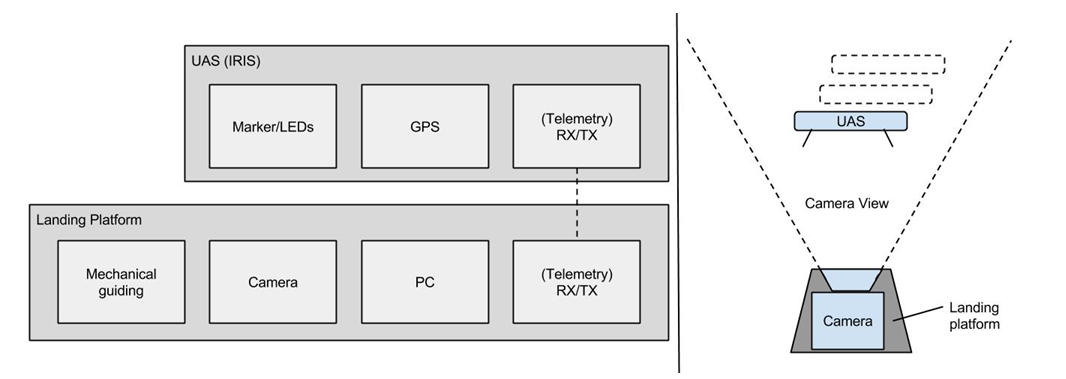
\includegraphics[width=0.8\textwidth]{imgs/introduction}
\end{center}
The picture above shows the basic idea of how the system could be build.

Link to demo video \url{https://youtu.be/I4g7Ij-pmPY}
%
\section{Mechanical design}
\input{mechanical/mechanical_design.tex}
%
\newpage
\section{ESC - Electronic Speed Controller}
\input{ESC/ESC-main.tex}
\input{ESC/ESC_basic_BLDC.tex}
\newpage
\input{ESC/ESC_electrical_equivalent.tex}
\input{ESC/ESC_Sensor_or_sensorless.tex}
\input{ESC/ESC_BEMF_Sensing.tex}
\input{ESC/ESC_Speed_control.tex}
\subsection{Motor driver circuit}
\input{ESC/ESC_driver_circuit.tex}
\input{ESC/ESC_circuit_power_stage.tex}
\input{ESC/ESC_circuit_ADC.tex}
\input{ESC/ESC_circuit_layout.tex}
%\subsubsection{Motor circuit conclusion}
%\input{ESC/ESC_circuit_conclusion.tex}
\subsection{FPGA implementation}
\input{ESC/ESC_FPGA_control_main.tex}
\input{ESC/ESC_VHDL_commutation_machine.tex}
\input{ESC/ESC_VHDL_subconclusion.tex}
%
\clearpage
\section{Position feedback}
\input{gyro_acc/gyro_acc-main.tex}
%
\clearpage
\section{Control algorithm}
\label{chapter:control_algorithm}
\input{control/control.tex}
%
\clearpage
\section{Wireless management}
\input{wireless/wireless-main.tex}
%
%
\subsection{Bluetooth implementation}\label{tosnetblue}
\label{subsec:bluetooth-implementation}
\input{wireless/bluetooth.tex}
%
\subsection{$\mu$TosNet over Bluetooth}
\label{subsec:tosnet}
\input{wireless/tosnet.tex}
%
\subsection{Graphical User Interface}
\input{wireless/gui.tex}
%
\subsection{Part conclusion}
\section{Conclusion}
Each part of this project partially works as a separate unit. However there were not enough time to make all ROS nodes communicate, and so the complete system was not tested together. All components need finalizing before the system can be used in agriculture.

The concept for a landing platform developed in this project is proven. The aircraft can be guided in place and successfully docked. However the prototype is indeed a prototype. The connector pods are too weak. The connector pads are made of aluminum foil which is fragile and not ideal in any way. Also the landing platform has to be protected against the environment somehow before it is ready for use in agriculture. 

Due to the brightness of the sky, the blob detection does not work outdoors at the tested distances. Blob detection work much better indoors; it is probable that blob detection might work at shorter distances than the tested distances. The shape detector works considerably better, with a worst case registered error rate of \SI{11}{\percent}. A better camera might be able to see the blob, allowing for all parts of the visual tracking system to work.

It was found that the Pixhawk module works well with both APM flight stack and Pixhawk flight stack. Problems with two software ground control stations were many, but QGroundControl works well with Ubuntu and APM Planner 2 works well with OS X. Different flight modes exist and AltHold, Auto and Land seems the best for automatic landing. The UAV and the RC-controller needs to be calibrated with a ground control station. When this is done correctly, both APM and Pixhawk flight stack showed good flight performance.

As the UAV is to take of by itself, weather must be taken into account. To do this METAR messages will be polled from the internet. 

MAVRos can be used to do offboard control of the UAV. RCoverride was tested and seems as a good solution for automatic landing. More testing needs to be done and an application using RCoverride to control the UAV needs to be made. Pseudocode for such a system is shown, but much more work needs to be put into the application in order to have something useful. 
%\subsection{Android application}
%\input{wireless/android.tex}
%
\section{Electronic design}
\input{system/electronic.tex}
%
%\subsection{Power supply}
%\input{supply/supply.tex}
%
\clearpage
\section{Conclusion}
\label{sec:conclusion}
\section{Conclusion}
Each part of this project partially works as a separate unit. However there were not enough time to make all ROS nodes communicate, and so the complete system was not tested together. All components need finalizing before the system can be used in agriculture.

The concept for a landing platform developed in this project is proven. The aircraft can be guided in place and successfully docked. However the prototype is indeed a prototype. The connector pods are too weak. The connector pads are made of aluminum foil which is fragile and not ideal in any way. Also the landing platform has to be protected against the environment somehow before it is ready for use in agriculture. 

Due to the brightness of the sky, the blob detection does not work outdoors at the tested distances. Blob detection work much better indoors; it is probable that blob detection might work at shorter distances than the tested distances. The shape detector works considerably better, with a worst case registered error rate of \SI{11}{\percent}. A better camera might be able to see the blob, allowing for all parts of the visual tracking system to work.

It was found that the Pixhawk module works well with both APM flight stack and Pixhawk flight stack. Problems with two software ground control stations were many, but QGroundControl works well with Ubuntu and APM Planner 2 works well with OS X. Different flight modes exist and AltHold, Auto and Land seems the best for automatic landing. The UAV and the RC-controller needs to be calibrated with a ground control station. When this is done correctly, both APM and Pixhawk flight stack showed good flight performance.

As the UAV is to take of by itself, weather must be taken into account. To do this METAR messages will be polled from the internet. 

MAVRos can be used to do offboard control of the UAV. RCoverride was tested and seems as a good solution for automatic landing. More testing needs to be done and an application using RCoverride to control the UAV needs to be made. Pseudocode for such a system is shown, but much more work needs to be put into the application in order to have something useful. 
%
\subsection{Possible development}
\input{conclusion/develop.tex}
%
\subsection{Robustness}
\input{conclusion/robustness.tex}
%
\newpage
%\bibliographystyle{IEEEtran}

\setstretch{1}

\setlength{\bibsep}{10pt}
\bibliographystyle{IEEEtran}
\bibliography{bibliography/bibliography}
%
\input{appendix/appendix.tex}
\input{appendix/appendix_boards.tex}
%
\end{document}